% Created 2020-07-16 Thu 12:21
% Intended LaTeX compiler: pdflatex
\documentclass[unicode, 12pt, aspectratio=43]{beamer}
\usepackage[utf8]{inputenc}
\usepackage[T1]{fontenc}
\usepackage{graphicx}
\usepackage{grffile}
\usepackage{longtable}
\usepackage{wrapfig}
\usepackage{rotating}
\usepackage[normalem]{ulem}
\usepackage{amsmath}
\usepackage{textcomp}
\usepackage{amssymb}
\usepackage{capt-of}
\usepackage{hyperref}
\usefonttheme{professionalfonts}
\usepackage[T1]{fontenc}
\usepackage[sort, compress]{natbib}
\let\realcitep\citep \renewcommand*{\citep}[1]{{\footnotesize\realcitep{#1}}}
\usepackage{url}
\usetheme{metropolis}
\setbeamertemplate{footline}{ \hfill \usebeamercolor[fg]{page number in head/foot} \usebeamerfont{page number in head/foot} \insertframenumber\kern1em\vskip2pt }
\setbeamertemplate{items}[default]
\setbeamertemplate{itemize item}{\small\raise0.5pt\hbox{$\blacksquare$}}
\setbeamertemplate{itemize subitem}{\footnotesize\raise1.5pt\hbox{$\bullet$}}
\setbeamertemplate{itemize subsubitem}{\scriptsize\raise1.5pt\hbox{$\blacktriangleright$}}
\setbeamertemplate{navigation symbols}{}
\usepackage{xltxtra}
\usepackage{booktabs}
\usepackage[absolute,overlay]{textpos}
\usepackage{pgfpages}
\XeTeXlinebreaklocale "ja"
\setsansfont{Noto Sans CJK JP}
\renewcommand{\baselinestretch}{1.3}
\usetheme{default}
\author{出口 祥之 <\texttt{deguchi@ai.cs.ehime-u.ac.jp}>}
\date{2020/07/16 二宮研 論文輪読会}
\title{Tree Transformer: Integrating Tree Structures into Self-Attention}
\subtitle{(Wang et al., EMNLP 2019)}
\institute{}
\hypersetup{
 pdfauthor={出口 祥之 <\texttt{deguchi@ai.cs.ehime-u.ac.jp}>},
 pdftitle={Tree Transformer: Integrating Tree Structures into Self-Attention},
 pdfkeywords={},
 pdfsubject={},
 pdfcreator={Emacs 26.3 (Org mode 9.1.9)}, 
 pdflang={English}}
\begin{document}

\maketitle

\begin{frame}[label={sec:org175c6f6}]{Links}
\begin{block}{Paper:}
\begin{itemize}
\item \url{https://www.aclweb.org/anthology/D19-1098/}
\end{itemize}
\end{block}
\begin{block}{Implementation:}
\begin{itemize}
\item \url{https://github.com/yaushian/Tree-Transformer}
\end{itemize}
\end{block}
\end{frame}

\begin{frame}[label={sec:orgeafaf79}]{Introduction}
\begin{itemize}
\item RNN では木構造を扱えるモデルが存在する (Tree-RNNs)
\item Transformer ベースのモデルで直接木構造を扱うモデルはない

\item シンプルなモジュールを追加するだけ
\begin{itemize}
\item 実装が簡単
\item 教師なし構文解析で良い性能
\item 人間の直感とも一致するような階層構造が得られる
\item 説明可能な Attention を持つようになる
\end{itemize}
\end{itemize}
\end{frame}

\begin{frame}[label={sec:orgaeaefe4}]{Tree Transformer}
\begin{center}
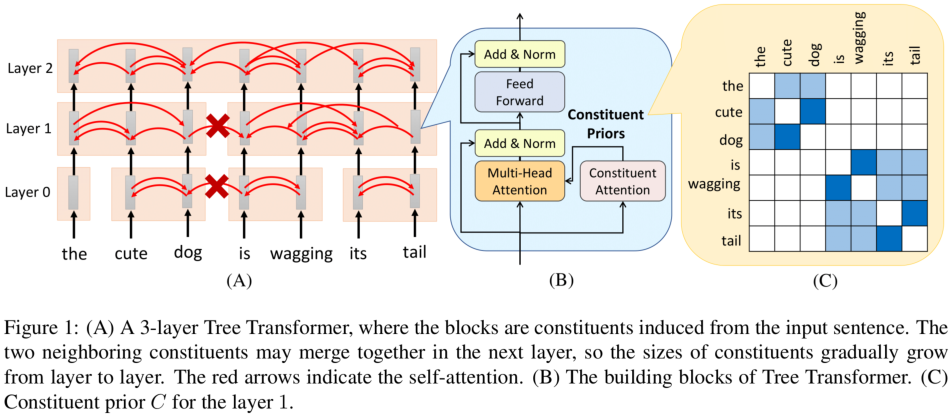
\includegraphics[width=\linewidth]{./figure/Figure1.pdf}
\end{center}
\end{frame}

\begin{frame}[label={sec:org5a00731}]{Constituent Prior}
\begin{columns}
\begin{column}{1.0\columnwidth}
\begin{block}{Attention 確率分布行列に Constituent Prior \(C\) を掛け合わせる}
\begin{itemize}
\item 通常の Transformer の確率分布行列 \(E\)
\begin{equation*}
  E = \mathrm{softmax}(\frac{QK^\top}{\sqrt{d_k}})
\end{equation*}

\item Tree Transformer の確率分布行列 \(E\)
\begin{equation*}
  E = C \odot \mathrm{softmax}(\frac{QK^\top}{\sqrt{d_k}})
\end{equation*}
※ \(\odot\) は要素積
\vspace{0.2cm}
\item \(C\) は Constituent Attention モジュール (後述) により計算される
\end{itemize}

\begin{textblock*}{0.3\linewidth}(265pt, 130pt)
    \centering
    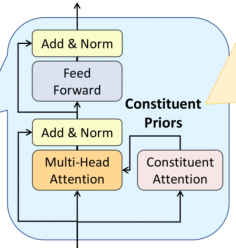
\includegraphics[width=\linewidth]{./figure/Figure1_b.pdf}
\end{textblock*}
\end{block}
\end{column}
\end{columns}
\end{frame}

\begin{frame}[label={sec:org69785e0}]{Constituent Attention}
\begin{columns}
\begin{column}{0.8\columnwidth}
\begin{block}{\(C\) を計算するモジュール}
\begin{itemize}
\item \(C_{i,j} (= C_{j, i})\) は単語 \(w_i\) から単語 \(w_j\) まで (\(w_j\) から \(w_i\) まで) が同じ構成要素である確率
\item 隣り合った単語が同じ構成要素である結合確率 \(a\) を後述の手法により計算 \\ \(a = \{a_1, \ldots, a_i, \ldots, a_N\}\)
\item \(a\) から \(C_{i,j} = \prod_{k=i}^{j-1} a_k\) を計算
\begin{itemize}
\item \(w_i\) 〜 \(w_j\) 間の中の \(a_{i \le k < j}\) の値が小さいときに \(C_{i,j}\) も小さくなるよう,\(C_{i, j}\) は和ではなく積で計算
\item 実際の計算では,勾配消失問題を回避するため \(\mathrm{logsumexp}\) により計算
\end{itemize}
\end{itemize}
\end{block}
\end{column}

\begin{column}{0.25\columnwidth}
\begin{center}
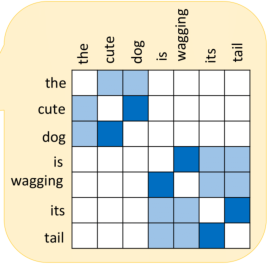
\includegraphics[width=1.0\linewidth]{./figure/Figure1_c.pdf}
\end{center}
\end{column}
\end{columns}
\end{frame}

\begin{frame}[label={sec:org1e1a03b}]{Neighboring Attention}
\begin{columns}
\begin{column}{1.1\columnwidth}
\begin{block}{各レイヤで \(a\) を計算}
\begin{enumerate}
\item \(w_i\) と \(w_{i+1}\) をそれぞれ \(d_{model}\) 次元の \(q_i\) と \(k_{i+1}\) に線形変換
\item スコア \(s_{i, i+1} = \frac{q_i k_{i+1}}{d_{model} / 2}\) を計算 \vspace{0.3cm}
\item \(p_{i, i+1}, p_{i, i-1} = \mathrm{softmax}(s_{i, i+1}, s_{i, i-1})\)
\begin{itemize}
\item \footnotesize \((p_{i, i+1} + p_{i, i-1}) = 1\) にしないと疎な分布にならないため重要 \normalsize
\end{itemize}
\item \(p_{i, i+1}\) と \(p_{i+1, i}\) の幾何平均より \(\hat{a}_i\) を計算
\begin{itemize}
\item \(C\) を対称行列にするため
\end{itemize}
\item Hierarchical Constraint (後述) に \(\hat{a}_i\) を渡して \(a_i\) を計算
\end{enumerate}

\begin{textblock*}{0.4\linewidth}(220pt, 110pt)
    \centering
    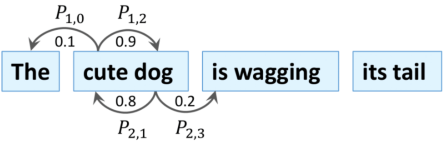
\includegraphics[width=\linewidth]{./figure/Figure2.pdf}
\end{textblock*}
\end{block}
\end{column}
\end{columns}
\end{frame}

\begin{frame}[label={sec:orgecf2472}]{Hierarchical Constraint}
\vspace{-2.5cm}
\begin{block}{レイヤ間の階層構造を構築}
\begin{itemize}
\item 上のレイヤほど構成要素の幅を広くする
\item レイヤ \(l\) ,位置 \(i\) の隣接単語の結合確率を \(a_i^l\) とすると, \(a_i^l = a_i^{l-1} + (1 - a_i^{l-1})\hat{a}_i^l\)
\begin{itemize}
\item なお, \(a_i^{-1} = 0\)
\item これにより制約 \(a_i^{l-1} < a_i^l\) がかかる
\end{itemize}
\item \(a^l\) から \(C^l\) を計算
\end{itemize}

\begin{textblock*}{0.45\linewidth}(190pt, 180pt)
    \centering
    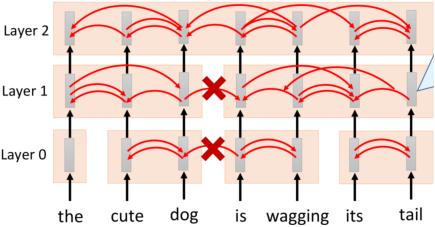
\includegraphics[width=\linewidth]{./figure/Figure1_a.pdf}
\end{textblock*}
\end{block}
\end{frame}

\begin{frame}[label={sec:org259673a}]{\large Unsupervised Parsing from Tree Transformer}
\begin{columns}
\begin{column}{0.5\columnwidth}
\begin{center}
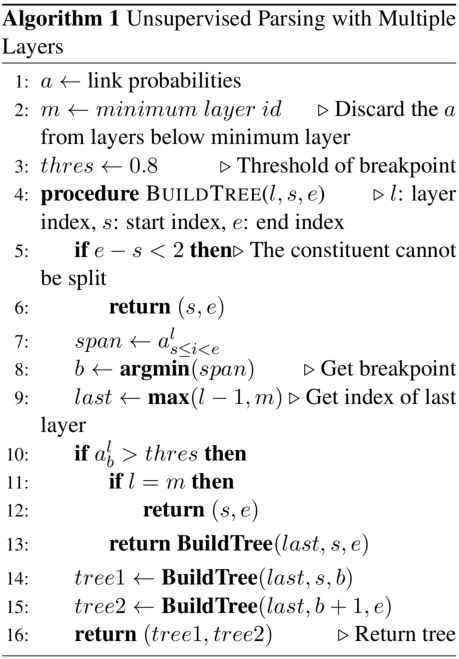
\includegraphics[width=\linewidth]{./figure/Algorithm1.pdf}
\end{center}
\end{column}

\begin{column}{0.6\columnwidth}
\begin{center}
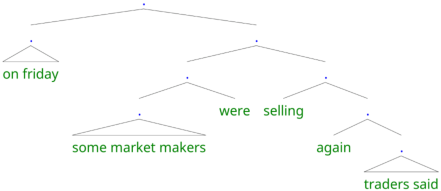
\includegraphics[width=\linewidth]{./figure/Figure3.pdf}
\end{center}
\end{column}
\end{columns}
\end{frame}

\begin{frame}[label={sec:org5344bc8}]{Experiments}
\begin{itemize}
\item モデルが木構造を捉えられるのか調べるため教師なし句構造解析により文法推論実験
\end{itemize}

\begin{center}
\begin{tabular}{ll}
\toprule
訓練データ & WSJ\\
訓練法 & Masked LM\\
評価データ & Penn Treebank (WSJ-test / WSJ-10)\\
\bottomrule
\end{tabular}
\end{center}
\end{frame}

\begin{frame}[label={sec:orge7938fb}]{Results}
\begin{block}{F1 スコア (WSJ-test / WSJ-10)}
\begin{columns}
\begin{column}{0.5\columnwidth}
\begin{block}{WSJ-test}
\begin{center}
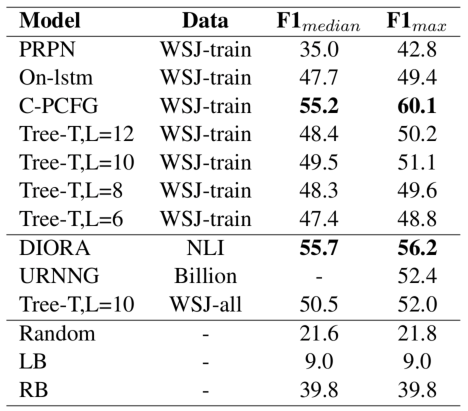
\includegraphics[width=\linewidth]{./figure/Table1.pdf}
\end{center}
\end{block}
\end{column}

\begin{column}{0.5\columnwidth}
\begin{block}{WSJ-10}
\begin{center}
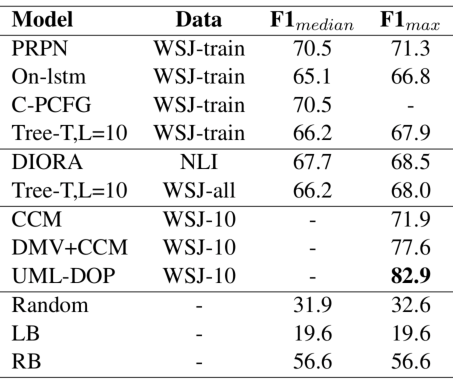
\includegraphics[width=\linewidth]{./figure/Table2.pdf}
\end{center}
\end{block}
\end{column}
\end{columns}
\end{block}
\end{frame}

\begin{frame}[label={sec:org6fd6632}]{Results}
\begin{block}{構成要素の Recall (各ラベルで比較)}
\begin{center}
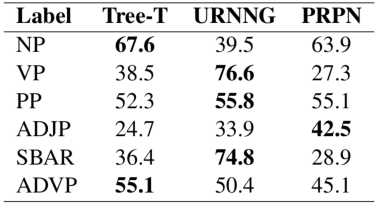
\includegraphics[width=0.5\linewidth]{./figure/Table3.pdf}
\end{center}
\end{block}
\end{frame}

\begin{frame}[label={sec:org2a42c67}]{Analysis}
\begin{center}
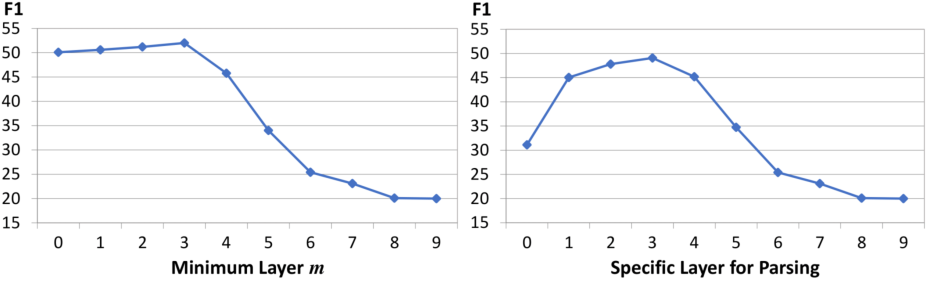
\includegraphics[width=\linewidth]{./figure/Figure4.pdf}
\end{center}
\end{frame}

\begin{frame}[label={sec:org5710da1}]{Interapretable Self-Attention}
\begin{center}
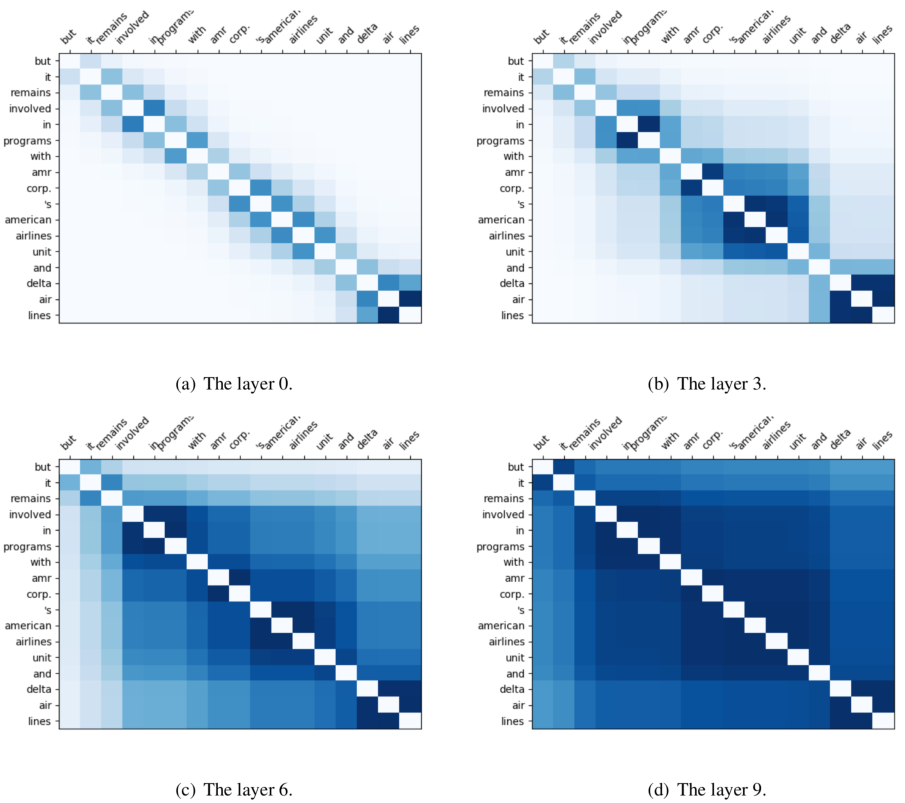
\includegraphics[width=0.8\linewidth]{./figure/Figure5.pdf}
\end{center}
\end{frame}

\begin{frame}[label={sec:orgec2598a}]{Masked Language Modeling}
\begin{block}{\texttt{[MASK]} トークンの perplexity を評価}
\begin{center}
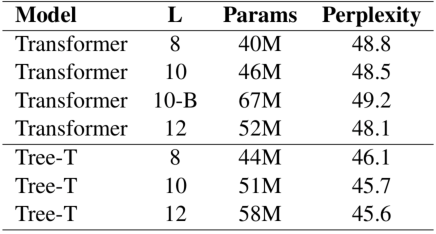
\includegraphics[width=0.5\linewidth]{./figure/Table4.pdf}
\end{center}
\begin{itemize}
\item perplexity は通常の Transformer ベースのモデルより Tree Transformer のほうが低い
\end{itemize}
\end{block}
\end{frame}

\begin{frame}[label={sec:org2b7f318}]{Limitations and Discussion}
\begin{itemize}
\item 訓練済み BERT でパラメタ初期化を行うと性能が酷く低下
\begin{itemize}
\item BERT の Attention が Tree Transformer と全く異なる構造を学習していることを示唆
\end{itemize}

\item この 1 文がよくわからなかった
\begin{itemize}
\item ``\textrm{In addition, with a well-trained Transformer, it is not necessary for the Constituency Attention module to induce reasonable tree structures, because the training loss decreases anyway.}''
\end{itemize}
\end{itemize}
\end{frame}

\begin{frame}[label={sec:org9ae1936}]{Conclusion and Future Work}
\begin{itemize}
\item \textbf{Conclusion}
\begin{itemize}
\item 木構造を Transformer に組み込む初めての試み
\item 提案手法の Constituent Attention により木構造を自動的に学習
\begin{itemize}
\item 隣接する単語の結合確率から相互に結び付ける
\end{itemize}
\item 教師なし構文解析の性能は一貫した木構造を捉えるという点でモデルの有効性を示した
\end{itemize}

\item \textbf{Future Work}
\begin{itemize}
\item Transformer で木構造を捉える方向性について検討する価値はある
\item 解釈可能な Attention はモデルが自然言語を処理する方法を説明し,将来のさらなる改善を導く
\end{itemize}
\end{itemize}
\end{frame}
\end{document}